\section{Durchführung}
\label{sec:Durchführung}
\begin{figure}[H]
  \centering
  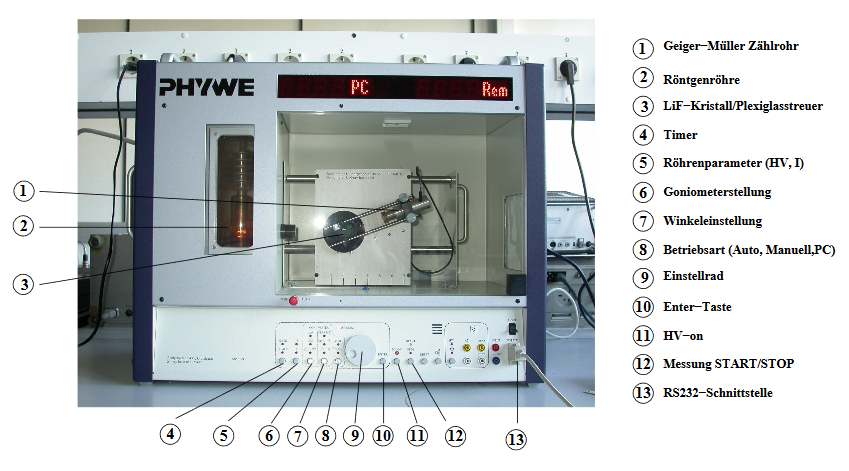
\includegraphics[height=5cm]{geraet.PNG}
  \caption{Abbildung des Röntgengeräts \cite{sample}.}
  \label{fig:geraet}
\end{figure}

Das in Abbildung \ref{fig:geraet} dargestellte Röntgengerät ist an einen PC
angeschlossen und wird mit dessen Hilfe bedient. Das Gerät besteht aus einer Cu-Röntgenröhre, welche
Röntgenstrahlung auf einen LiF-Kristall schießt. Dieser befindet sich in einem bestimmten Winkel
zu der einfallenden Strahlung. Hinter dem Kristall befindet sich dann ein Geiger-Müller-Zählrohr, welches
in einem bestimmten Abstand um den Kristall rotieren kann. Das Geiger-Müller-Zählrohr und
der Kristallwinkel können mit dem PC gesteurt werden und die gemessenen Daten
werden auf dem Bildschirm ausgegeben.
Zu Beginn wird eine Messung durchgeführt, bei welcher der Kristallwinkel konstant
bleibt. Das Zählrohr wird so programmiert, dass es den Bereich des durch den
Kirstall entstehenden Intensitätsmaximums abfahren sollte (Mit Integrationszeit von 5s).
Nach Ausgabe der Werte auf dem Bildschirm wird überprüft ob das Maximum tatsächlich an der
erwarteten Stelle auftritt und die Apparatur somit richtig justiert ist. Das Ergebnis der
Messung wird abgespeichert.
Anschließend wird das Röntgengerät in den 2:1 Koppelmodus (Kristallwinkel halb so
groß wie Winkel des Zählrohrs) geschaltet.
Nun wird das Emissionsspektum des Kupfers gemessen, indem man die Apparatur
die Intensitätsverteilung der Strahlung in einem entsprechenden Winkelbereich
Messen lässt. Die Ergebnisse werden wiederum abgespeichert.
Ähnlich wird das Absorptionsspektrum einiger Stoffe gemessen. Die Durchführung unterscheidet
sich lediglich darin, dass ein Plättchen des entsprechenden Stoffs vor das Zählrohr
gehängt wird und die Integrationszeit auf 20s erhöht wird. Sodann wird der zu messende
Winkelbereich eingestellt und die Messung gestartet. Dies wird für insgesamt vier
Stoffe durchgeführt.
